\documentclass{article}
\usepackage{styles/iclr2027/iclr2027_conference,times}
\usepackage[T1]{fontenc}
\usepackage{amsmath,amssymb,booktabs,tabularx,graphicx,placeins}
\usepackage{xcolor,listings,etoolbox}
\usepackage[hidelinks]{hyperref}
% Self-contained highlighting: no shell escape, Pygments or generated cache.
\definecolor{tigakeyword}{HTML}{174B8A}
\definecolor{tigastring}{HTML}{8C3B12}
\definecolor{tigacomment}{HTML}{52616B}
\definecolor{tigatype}{HTML}{087568}
\definecolor{tigacodebg}{HTML}{F7F9FC}
\lstdefinestyle{tigacode}{
  basicstyle=\small\ttfamily,
  keywordstyle=\color{tigakeyword}\bfseries,
  keywordstyle=[2]\color{tigatype},
  commentstyle=\color{tigacomment}\itshape,
  stringstyle=\color{tigastring},
  backgroundcolor=\color{tigacodebg},
  breaklines=true,columns=fullflexible,keepspaces=true,
  showstringspaces=false,upquote=true,tabsize=4,
  frame=single,rulecolor=\color{black!15},framesep=5pt,
  aboveskip=0.8em,belowskip=0.8em}
\lstdefinelanguage{TigaIR}{
  sensitive=true,
  alsoletter={._},
  morekeywords={module,func.func,return,arith.mulf,arith.addf,gf.apply,
    gf.yield,gf_iter.traverse,gf_kernel.launch,gf_storage.transfer,
    gf_storage.release,gf_storage.join},
  morekeywords=[2]{f16,f32,f64,i1,i32,i64,index,tensor,memref,
    block_rows,block_neighbors,num_warps,pipeline_stages},
  morecomment=[l]{//},
  morestring=[b]"}
\lstdefinelanguage{TigaShell}{
  sensitive=true,alsoletter={-},
  morekeywords={gf-opt},
  morekeywords=[2]{-gf-lower-domain-to-iter,-gf-lower-iter-to-kernel,
    -gf-select-kernel-schedule,-gf-plan-distributed-tasks},
  morecomment=[l]{\#},morestring=[b]",morestring=[b]'}
\lstset{style=tigacode}

\newcommand{\code}[1]{\texttt{#1}}
\newcolumntype{Y}{>{\raggedright\arraybackslash}X}
\title{Tiga: Compiling Graph\\Message Passing at Scale}
\author{Anonymous authors}
\hypersetup{pdfauthor={},pdftitle={Tiga: Compiling Graph Message Passing at Scale},
pdfsubject={ICLR 2027 workshop manuscript draft; not submitted}}
% Keep official layout and anonymous mode, but never imply an actual submission.
\makeatletter
\patchcmd{\@maketitle}{Paper under double-blind review}{Workshop manuscript draft}
  {}{\PackageError{tiga}{Cannot replace template review status}{Check template version}}
\makeatother
\begin{document}
\maketitle
\lhead{ICLR 2027 workshop manuscript draft --- not submitted}
\begin{abstract}
Graph message passing is a common computational pattern in learning and
numerical simulation, but explicit graph construction and edge-wise tensor
operations can consume more memory than the final result. We present Tiga,
a just-in-time compiler that keeps graph relations and reduction semantics
visible until traversal and execution are selected. Generated relations can
be consumed by aggregation without storing a complete edge list or message
array. For explicit graphs that exceed device memory, a paged runtime streams
topology and source fields through host memory while retaining a bounded
temporary device working set. The interface accepts ordinary PyTorch tensors,
with path-specific automatic differentiation and native storage controls for
offloaded execution. Experiments compare forward latency and allocation with
matched Torch and PyTorch Geometric implementations, and demonstrate billion-edge
forward execution on a memory-limited GPU. The results motivate relation-aware
compilation while exposing the host-staging costs of capacity-oriented paging.
Gradient checks establish supported derivative semantics separately from the
forward-performance measurements.
\end{abstract}
\section{Introduction}
Message passing describes computation through entities, interactions, local
functions and reductions. In machine learning, this pattern includes graph
neural networks, point-cloud neighborhoods and attention; numerical simulation
uses related structures for particles and mesh operators. The same high-level
pattern can require very different execution strategies. A stored sparse graph
needs indexed traversal, a radius relation can exploit spatial locality, and
a dense relation need not have an explicit edge array at all.

Tensor-oriented implementations often build connectivity first, gather fields
for every edge, compute messages, and finally reduce them. For edge count
and feature width denoted by $E$ and $F$, a materialized message array uses
storage proportional to $EF$, even when its sole consumer produces $NF$
output values for $N$ destinations. Dynamic coordinates can make the cost of
constructing these intermediates recur at every call. When the input graph
itself exceeds device memory, fusion alone is insufficient: execution must
also control which topology and field pages reside on the accelerator.

Tiga, short for \emph{Target-Independent Graph Acceleration}, separates the
meaning of a message-passing program from its traversal, hardware mapping and
storage residence. Target independence describes this separation, not equal
backend coverage: current executable routes target CPUs and NVIDIA GPUs.
The central design choice is to retain relation and reducer information before
lowering to tensor and device operations. This enables two complementary
mechanisms: consuming generated neighbors directly, and streaming stored
graphs with a bounded temporary working set.

This paper contributes a relation-aware compilation interface and lowering
strategy, a destination-page execution contract for graphs exceeding device
memory, and an evaluation of their forward latency, allocation and capacity.
The results establish useful execution paths rather than a universal framework
ranking. In particular, the evaluation does not isolate every compiler
optimization or establish end-to-end training throughput. Differentiation and
distributed execution are supported on specific paths, with their boundaries
stated separately from the central performance claims.

\paragraph{Relation to prior systems.}
PyTorch Geometric exposes message passing to graph-learning applications
\citep{pyg,pyg2}. Graphiler retains graph-related dataflow to eliminate redundant
work and storage \citep{graphiler}; FeatGraph composes sparse traversal and
feature schedules \citep{featgraph}; Seastar generates fused forward/backward
kernels \citep{seastar}; and GALA composes graph-training transformations
\citep{gala}. Tiga likewise exploits message semantics, but additionally retains
generated relation constructors and explicit storage residence in its execution
model. These design differences are not comparative performance claims against
those compilers. GraphIt separates algorithms from schedules \citep{graphit},
while TACO and SparseTIR separate sparse iteration and storage choices
\citep{taco,sparsetir}. GraphChi and X-Stream establish that partitioned streaming
can make large graphs executable on a single machine \citep{graphchi,xstream}.
Tiga builds on these principles for differentiable numerical field programs;
neither fusion nor offloading is claimed as a new idea in isolation.

\section{Relation-aware compilation and bounded execution}
\label{ws:design}
\subsection{The program retains interactions, not edge arrays}
A graph maps each edge to a source and a destination. A message function reads
source, destination and edge fields; a reducer combines messages for each
destination. The result is
$$
y_i=\operatorname{finalize}\!\left(
\bigoplus_{e:d(e)=i}\operatorname{lift}
\big(f(x_{s(e)},z_i,a_e;\theta)\big)\right).
$$
The reducer declares an identity, state update and finalization. Duplicate
edges are separate contributions; empty rows follow the reducer's identity
and finalization convention. An optional node function consumes the reduced
value. The edge function determines what is computed, while the graph determines
which interactions exist.

For example, this program sums source features over a coordinate-dependent
radius relation. Positions and features are ordinary Torch tensors on the same
device; rows denote destinations and columns denote sources.
\begin{lstlisting}[language=Python]
import tiga as tg

class NeighborSum(tg.MessagePassing):
    reducer = tg.sum()
    def edge(self, src, dst, edge):
        return src.x

graph = tg.Graph.radius(positions, cutoff=0.1)
y = NeighborSum()(graph=graph, src={"x": x}, dst={})
\end{lstlisting}
The interface does not require an edge list, although a consumer may select an
explicit representation. Dense and triangular graphs similarly describe an
interaction domain. For causal attention, the destination supplies a query,
the source supplies a key/value, and an online-softmax reducer combines score
and value messages. Preserving the reducer state admits streaming evaluation
without a global score matrix, following the IO-aware principle exemplified by
FlashAttention \citep{flashattention}.

\subsection{Lowering preserves legality before choosing a schedule}
Tiga uses MLIR for its compiler representations \citep{mlir}. Domain IR retains
field roles, graph construction and message/reducer regions. Iter IR introduces
relation-coordinate traversal. Kernel IR assigns tiles and reduction work to
execution resources. Task/Storage IR describes dependencies, physical copies
and ownership where the selected path needs them. Tensor IR carries numerical
expressions alongside these layers; it is not a mandatory final stage.

Three properties constrain the transformations. First, field roles distinguish
a source ID from an edge position, even when both index floating-point arrays.
Second, reducer associativity permits regrouping and commutativity permits
reordering; arbitrary Python functions do not automatically satisfy either
property. Third, shape, dtype, layout and topology guards determine whether an
executable remains legal. Floating-point reduction changes require numerical
tolerances even when real-arithmetic semantics agree. NVIDIA lowering emits
serialized Triton IR for provider compilation \citep{triton}; native CPU paths
lower through LLVM. A provider interface alone does not establish a working
backend on another vendor's hardware.

\paragraph{Generated relations.}
For supported low-dimensional Euclidean radius workloads, a cell directory
limits traversal to neighboring cells. An exact distance predicate selects
accepted sources, whose fields can be consumed immediately by the reduction.
This avoids storing accepted-edge indices, distances and messages globally.
A custom metric needs a compatible spatial bound before that traversal is legal.

For exact kNN, a destination program scans candidate tiles and keeps a padded
top-k state, ordered by squared distance and source ID. If the smallest key
in a candidate tile cannot improve the retained state, sorting and merging
that tile are skipped; its distances are still computed. This is exact
selection pruning, not approximate neighbor search or a subquadratic algorithm.
Compatible new coordinates can rebind an existing executable without capture
and lowering. Coordinates remain live inputs: executable reuse never implies
reuse of previously selected neighbors.

\subsection{Paging separates capacity from kernel speed}
\label{ws:paging}
Explicit graphs larger than device memory use a native storage path. Topology
and source fields remain in a persistent store. The runtime loads a bounded
destination-row page, gathers its source fields on the host, stages the page
to CUDA and runs its reduction. It assembles the final output in a resident
device tensor. The capacity constraint is therefore
$$
M_{\mathrm{output}}+M_{\mathrm{active\ topology}}
+M_{\mathrm{staged\ fields}}+M_{\mathrm{temporary}}
\le B_{\mathrm{device}},
$$
where the budget applies to Tiga-managed device buffers, not other processes
or the full CUDA context. The output must still fit the device. Page topology
and field versions must agree; transfer must finish before consumption; and
storage cannot be recycled until its consumers finish.

The current implementation gathers features in page-edge order, potentially
repeating a source value many times. It also returns completed output pages
through host bytes before writing the resident result. These choices bound
temporary memory but can dominate runtime. The measured configuration is
serialized, without prefetch. Optional read-ahead does not implement a complete
disk--host--device overlap pipeline. Ordinary Torch tensors remain under Torch's
allocator; Tiga-managed paging uses native tensors rather than silently taking
ownership of arbitrary Torch storage.

\paragraph{Differentiation boundary.}
Supported Torch-facing programs interoperate with Torch autograd. CUDA EdgeNN
paths recompute local activations in a symbolic vector--Jacobian product (VJP);
some other compiled forwards replay Torch operations during backward. CPU
paging has a supported native VJP, but CUDA paged execution and the dense
streaming attention path evaluated here have no compiled backward. Derivatives
act on the selected relation, not discrete radius membership or kNN selection.
Appendix~\ref{ws:gradients} distinguishes the numerical checks from training
performance evidence.

\section{Evaluation}
\label{ws:evaluation}
\paragraph{Setup.}
The main host has a Ryzen 7 255, approximately 44 GiB RAM, NVMe storage and an
RTX 5070 Ti with 16 GiB device memory. Software comprises Torch 2.11.0+cu128,
Triton 3.6.0, PyG 2.8.0.post1, pyg-lib 0.9.0+pt211cu128 and driver 595.84.
These are shared, non-clock-locked hosts. Timings are synchronized host wall
time through completed output. The comparisons use ordinary Torch inputs;
paging and distributed runs use native tensors. All performance results are
FP32 forward evaluations, not training steps. Figure~\ref{ws:performance}
shows matched shapes and semantics, with lower latency and allocation preferable.

\subsection{Generated and stored relations}
Stored CSR uses degree 32 and 32 features at 8,192--131,072 nodes. Baselines
are Torch sparse multiplication and PyG COO gather--scatter. Dynamic radius
uses a scalar distance-weighted sum, nominal degree 32 and the same node sizes.
Dynamic kNN uses a scalar neighbor sum with $k=16$ at 1,024--131,072 points.
Each dynamic call changes coordinates, constructs the relation and consumes
it; unchanged-input topology caching is not timed as construction.

PyG baselines use their respective radius/kNN builder plus COO message passing.
Pure Torch baselines compute distances in bounded row chunks and then use
CSR/sparse multiplication for radius, or top-k followed by gather/sum for kNN.
The distance-block budget is 16,777,216 pairs. These eager all-pairs baselines
do not represent the best possible spatial-index implementation in Torch.
Complete explicit-reference/PyG edge sets agree for both coordinate snapshots.
Radius inputs avoid ambiguous floating-point cutoffs, and the neighbor cap
does not truncate the measured relations.

Each of 36 configurations runs in a fresh process, with provider order
randomized, four warmups and ten timed calls checked at relative and absolute
tolerance $3\cdot10^{-4}$. Curves show medians and sample ranges. Peak
Torch-allocated bytes include inputs, output, graph representations and
temporaries, but exclude allocator reserve, CUDA context and other processes.
Largest-shape audits found no extra Tiga-native device-buffer allocation on
these Torch paths. Compilation is outside the warm timing window.

\begin{figure}[t]
\centering
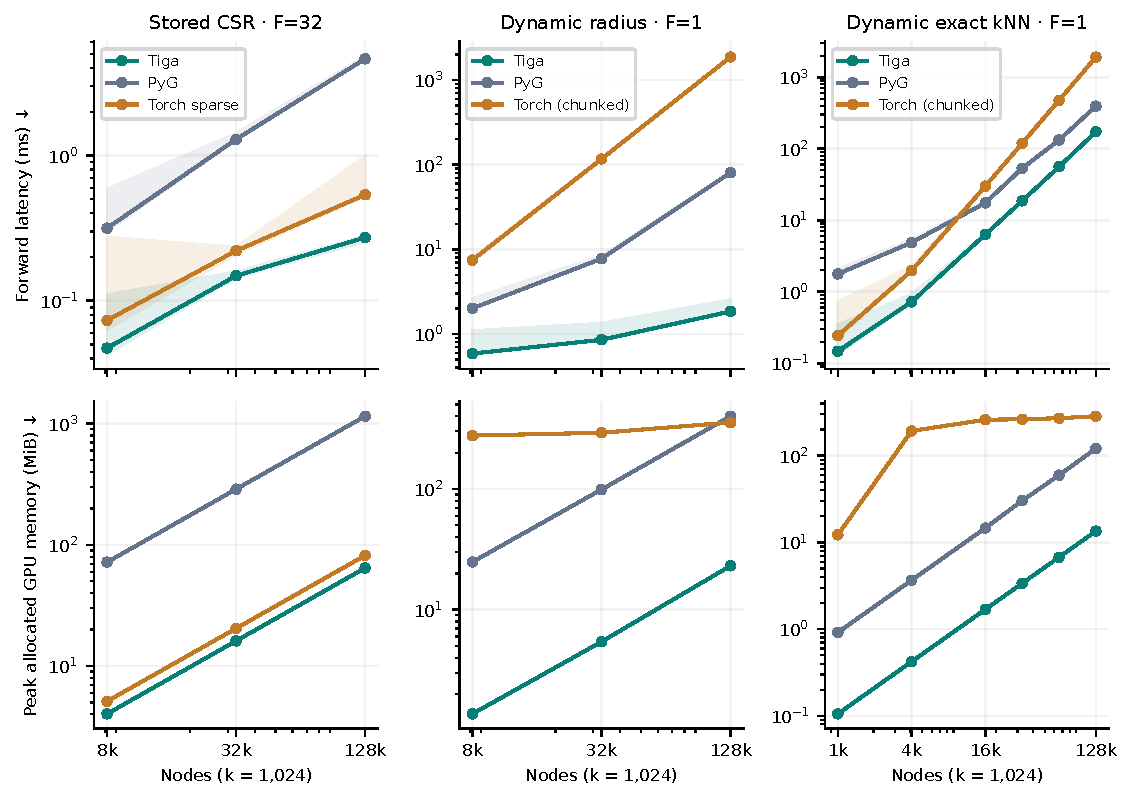
\includegraphics[width=\linewidth]{figures/q1-performance-memory.pdf}
\caption{Matched forward latency and allocated GPU memory. Columns are distinct
workloads: stored CSR has 32 features, dynamic radius and kNN have one.
Both axes are logarithmic. Dynamic calls include rebuilding from changed
coordinates; Torch (chunked) uses a pure Torch builder and aggregation.}
\label{ws:performance}
\end{figure}

Stored CSR achieves 1.49--1.97$\times$ speedup and approximately 1.27$\times$
lower allocation than Torch sparse across the three sizes. At 131,072 radius
points, Tiga takes 1.84 ms versus 80.24 ms for PyG and 1,870.09 ms for chunked
Torch, with allocation of 23.14, 400.22 and 355.01 MiB respectively. This
comparison combines algorithmic traversal choices and materialization/fusion
effects; it does not isolate the contribution of any one compiler pass.

At 131,072 kNN points, Tiga takes 172.37 ms versus 393.21 ms for PyG and
1,908.43 ms for chunked Torch; the allocations are 13.50, 121.13 and 285.00 MiB.
The PyG-relative speedup ranges from 2.28$\times$ to 12.06$\times$ over six
sizes. These results concern scalar messages on the tested geometries, not
wide-feature EdgeNNs or arbitrary point distributions.

\subsection{Billion-edge capacity and its cost}
The capacity workload explicitly stores a periodic directed CSR graph with
16 neighbors per destination and 32 features. The sweep contains 10M, 100M
and 1B edges with three fresh-process calls per size. Ingest is excluded;
forward includes loading, staging, compilation as encountered, computation
and output assembly. All output values are checked after timing against a
closed-form oracle; the execution still traverses every stored edge.

Pages contain 65,536 destination rows, the managed-device budget is 12 GiB,
and prefetch is disabled. At 1B edges, the graph has 62.5M nodes. Int64 CSR,
source and output together require at least 22.82 GiB for full residency
(18.86 GiB with int32 CSR), exceeding device capacity. These are calculated
lower bounds, not measured baseline OOMs.

\begin{figure}[t]
\centering
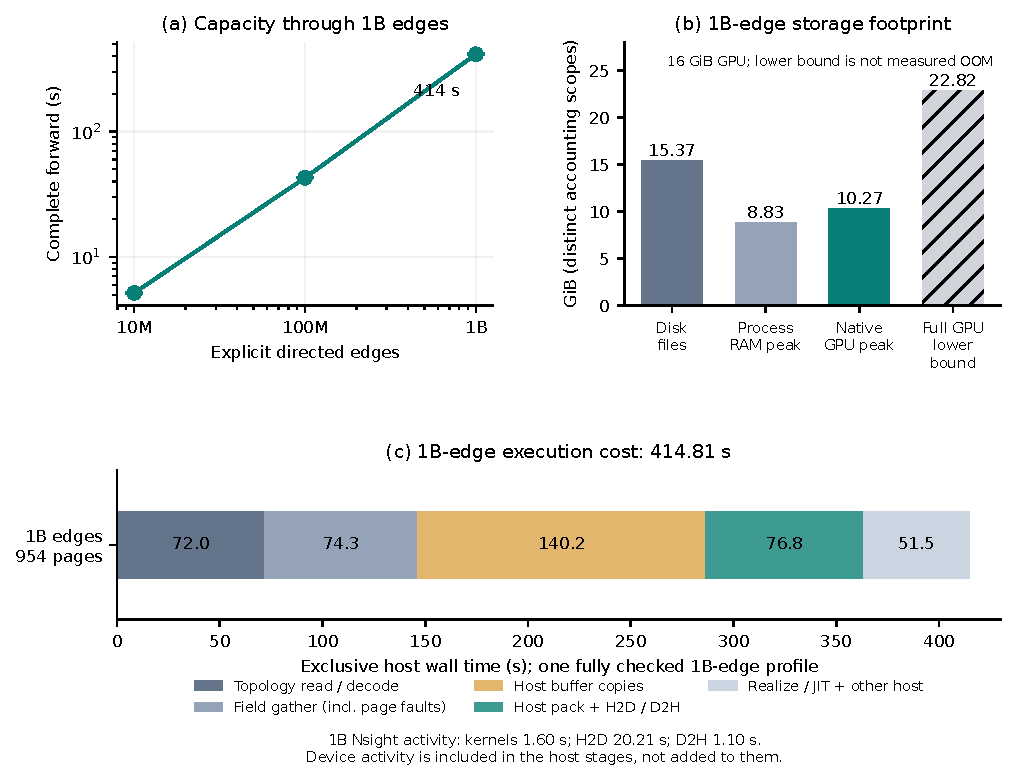
\includegraphics[width=\linewidth]{figures/q2-capacity-cost.pdf}
\caption{Capacity through 1B explicit edges. The full-residency requirement is
calculated; other memory bars have distinct measured accounting scopes.
The host-stage breakdown is one separately instrumented forward call, not
extra time added to the three-trial capacity sweep.}
\label{ws:capacity}
\end{figure}

The 1B median is 414.25 s (411.36--415.61), with maximum native GPU peak
10.27 GiB and forward process RSS 8.83 GiB. Disk topology/source storage is
15.37 GiB, and the resident output alone is 7.45 GiB. Sampled device-wide
usage, including unrelated services and pools, reaches 13.25 GiB.

A separate checked 1B profile spends 414.81 s in its forward window:
71.98 s topology read/decode, 74.27 s field gathering, 140.22 s host-buffer
copying, 76.79 s packing/transfers and 51.55 s setup/assembly/other work.
Nsight records 1.60 s of CUDA kernels and 20.21 s H2D activity inside those
host intervals. Source expansion turns 8 GB of stored features into 128 GB
of gathered values. Host staging, not reduction arithmetic, dominates.
The result establishes execution beyond device memory, not optimal offload
performance, capacity beyond host RAM, or a maximum supported edge count.
A hand-chunked peer could also trade storage traffic for capacity.

\paragraph{Distributed scope.}
For a separate two-host spatial-mesh experiment, a 5070 Ti and 4070 Ti SUPER
each own half the destination rows and exchange a one-layer halo through
NCCL Socket transport before local computation. At 22.51M directed edges,
paired-rank latency is 44.22 ms, versus 23.00 ms on the faster GPU alone.
Thus the current fixed partition does not establish a distributed speedup,
despite only 1.125 MiB of halo traffic. Appendix~\ref{ws:distributed} gives
the timing conditions and interpretation.
\FloatBarrier

\section{Discussion and conclusion}
Relation-aware compilation can reduce work and storage that arise from
prematurely expanding interactions. The performance measurements support this
opportunity for selected generated-relation workloads. Paging addresses a
different constraint: it makes an explicit billion-edge computation executable
on a memory-limited GPU, while exposing substantial host-staging overhead.
These mechanisms benefit from a shared separation of relation semantics,
traversal and storage, but neither makes every graph program efficient.

The present evidence leaves three important questions open. A same-search
materialized-versus-fused ablation is needed to separate traversal gains from
intermediate elimination. Real-data, wide-feature applications and complete
forward/backward steps are needed to establish learning-workload benefits.
Finally, first-call compilation costs and amortization need to be reported
alongside warm execution. Capacity comparisons additionally need a matched
bounded-memory baseline before claiming an advantage over manual chunking.
These missing measurements limit attribution and generalization; the reported
curves do not substitute for them.

The implementation also has path-dependent differentiation and backend coverage.
CUDA paging remains forward-only, output storage must fit the device, and
distributed ownership is fixed. The current results motivate improving source
staging and output assembly, and assessing load-aware partitioning rather than
assuming that a small halo guarantees strong scaling. Tiga provides a concrete
substrate for exploring these choices without changing the local message and
reducer interface.

\label{ws:main-end}
\clearpage
\section*{Reproducibility statement}
Section~\ref{ws:evaluation} and Appendix~\ref{ws:protocol} specify workloads,
timing boundaries, validation and allocation accounting. Figures are generated
from stored execution records with source/compiler hashes and configuration
checks; they are not predictions. The numerical examples distinguish compiled
forward execution from semantic gradient replay. No new measurement is inferred
from replotting an existing record.

\section*{AI use statement}
AI coding and writing assistants were used in software implementation and
testing, experiment design and tooling, literature discovery, interpretation
of measurements, figure/code preparation, and manuscript drafting and revision.
The numerical results reported here originate from recorded program executions,
not generated estimates. Automated numerical and provenance checks were used
to validate outputs, gradients on supported paths, and the recorded evidence.
The human author is responsible for the final content, attribution and claims.

\bibliographystyle{styles/iclr2027/iclr2027_conference}
\bibliography{references}
\clearpage
\appendix
\section{Experimental protocol and interpretation}
\label{ws:protocol}
\paragraph{Stored and dynamic comparisons.}
Stored CSR excludes relation construction from timing. PyG's COO representation
is included in its allocation; Torch sparse provides a peer that does not
materialize COO messages. Radius nominal degree is 32, with a cap of 128
verified not to truncate either coordinate snapshot. kNN excludes self-edges
and uses direct squared differences in the reference, avoiding a matrix-product
distance identity at close separations. Every timed output is checked outside
the measurement window. Sample ranges describe variation within the retained
calls, not cross-process confidence intervals. The dynamically generated cases
have one feature; the stored CSR and capacity cases have 32.

\paragraph{Capacity accounting.}
Topology and source files occupy 16.50 GB (15.37 GiB). The 1B graph's
two-billion-scalar output is checked exactly after each retained run. Native
device counters do not include unrelated allocations; process RSS is not total
machine RAM consumption; and disk footprint is not a simultaneous resident
allocation. The profiled outer call takes 417.05 s including profiler start/stop,
whereas the inner window takes 414.81 s. Exclusive host intervals sum to the
inner window. Device kernel/copy activity lies within these intervals and must
not be added again. mmap gathering includes page-fault IO, so it is not a
pure disk-service timer. The graph fits host RAM. Measured H2D traffic is
144.50 GB and D2H traffic is 8 GB; repeated source gathers explain why transfer
volume exceeds the stored input size.

\section{Differentiation checks}
\label{ws:gradients}
The EdgeNN check constructs a radius graph on 128 three-dimensional positions.
Each message concatenates source features of width eight and the displacement
from destination to source, applies an 11--16--4 ReLU MLP, and sums at the
destination. The loss is the mean squared output. An explicit Torch gather,
the same MLP parameters and destination \code{index\_add} provide a reference.
Output, source-feature, position and parameter gradients are compared; the
position derivative acts on displacements for the selected edges, not radius
membership. Using the same resolved graph isolates message and gradient
semantics rather than independently validating the neighbor search.

The attention check uses the exact triangular relation, two heads of width 64,
and an online-softmax reducer. CUDA streaming output is compared with explicit
FP32 Torch scores, causal masking, softmax and value multiplication. A separate
\code{program.reference} call checks query/key/value gradients against independent
Torch leaf tensors under a random output cotangent. This reference materializes
edges and messages. It is not a streaming backward kernel. Checks cover sequence
lengths 1, 7 and 65 on CPU, and 1, 7, 65 and 128 on CUDA, including singleton
and partial-tile cases. These tests establish first-order agreement, not
training throughput or universal higher-order differentiation.

\section{Distributed negative result}
\label{ws:distributed}
Nonperiodic hexahedral meshes of side lengths 32, 64 and 96 connect nodes
sharing an element in both directions without self-edges: 797,816, 6,596,856
and 22,508,920 directed edges. A 16-feature neighbor sum is evaluated, not a
complete FEM solve. Equal destination partitions exchange one interface layer
across a spatial plane; the boundary-row fraction falls from 6.25\% to 2.083\%.

Both hosts run matching compiler/runtime sources and NCCL 2.28.9 Socket
transport. Two warmups precede five changed-input calls; the median is taken
over paired-rank maximum durations. Timing includes exchange, scheduling,
computation and synchronization, but excludes topology setup, the control
barrier and checking. Replicated topology setup does not demonstrate
distributed topology capacity beyond one GPU.

At the largest size, full-graph medians are 89.75 ms and 23.00 ms on the two
cards, versus 44.22 ms distributed. Existing services occupy roughly 3 GiB on
the main host and 12 GiB on the Ubuntu/WSL second host. Hardware, environment
and contention are not independently controlled; the gap cannot be attributed
solely to GPU compute throughput. This is a deployment-specific result, not a
universal limit of graph partitioning.

\end{document}
